%| Weekly report template for CSUS Senior Design
%|
%| language: LaTeX
%| Author: Ben Smith
%| 
%| This source has been tagged with the "<CHANGE" tag in areas
%| that require updating when making a new docuent
%|
%| This source will generate a PDF file complete with thumbnails navigation menu and metadata.
%| Much of the tex awesomeness comes from http://www.michaelshell.org/ praise be to him for creating the guide

\documentclass[12pt,journal]{IEEEtran}

\newcommand{\TITLE}{Lab Three: Introduction to Verilog}
\newcommand{\KEYWORDS}{Logic Gates, Verilog, FPGA, Signaltap, Synthesis}
\newcommand{\ABSTRACT}{Two input logic gates are synthesized for the Altera Cyclone IV FPGA using the Quartus IDE. The logic gates are verified using a System Verilog testbench and Mentor's Modelsim HDL simulator}

%| Override compsoc class' Palatino font for body text, restores to Times New Roman
\renewcommand{\rmdefault}{ptm}\selectfont

%| IEEE Citation package
\usepackage{cite}

\usepackage[cmex10]{amsmath}        %| Asmerican Mathematical Society package for fancy maths  
\interdisplaylinepenalty=2500       %| Restores IEEE line spacing after amsmath

%| Better tables than LaTeX 2e
\usepackage{array}
\usepackage{graphicx}
\usepackage{float}
\usepackage{url}                    %| Improved URL handling
\usepackage{minted}
\usepackage{etoolbox}
%\AtBeginEnvironment{minted}{\singlespacing
%    \fontsize{9}{p}\selectfont}
\usepackage{listings}
\definecolor{mygreen}{rgb}{0,0.6,0}
\definecolor{ltgray}{rgb}{0.9,0.9,0.9}
\definecolor{dkgray}{rgb}{0.5,0.5,0.5}
\definecolor{mymauve}{rgb}{0.58,0,0.82}
\lstset{ %
  backgroundcolor=\color{ltgray},  % choose the background color; you must add \usepackage{color} or \usepackage{xcolor}
  basicstyle=\scriptsize\ttfamily,        % the size of the fonts that are used for the code
  breakatwhitespace=false,         % sets if automatic breaks should only happen at whitespace
  breaklines=true,                 % sets automatic line breaking
  captionpos=b,                    % sets the caption-position to bottom
  commentstyle=\color{mygreen},    % comment style
  deletekeywords={...},            % if you want to delete keywords from the given language
  escapeinside={\%*}{*)},          % if you want to add LaTeX within your code
  extendedchars=true,              % lets you use non-ASCII characters; for 8-bits encodings only, does not work with UTF-8
  frame=single,                    % adds a frame around the code
  keepspaces=true,                 % keeps spaces in text, useful for keeping indentation of code (possibly needs columns=flexible)
  keywordstyle=\color{blue},       % keyword style
  language=SystemVerilog,                % the language of the code
  morekeywords={*,...},            % if you want to add more keywords to the set
  numbers=left,                    % where to put the line-numbers; possible values are (none, left, right)
  numbersep=5pt,                   % how far the line-numbers are from the code
  numberstyle=\tiny\color{dkgray}, % the style that is used for the line-numbers
  rulecolor=\color{black},         % if not set, the frame-color may be changed on line-breaks within not-black text (e.g. comments (green here))
  showspaces=false,                % show spaces everywhere adding particular underscores; it overrides 'showstringspaces'
  showstringspaces=false,          % underline spaces within strings only
  showtabs=false,                  % show tabs within strings adding particular underscores
  stepnumber=1,                    % the step between two line-numbers. If it's 1, each line will be numbered
  stringstyle=\color{mymauve},     % string literal style
  tabsize=2,                       % sets default tabsize to 2 spaces
  title=\lstname                   % show the filename of files included with \lstinputlisting; also try caption instead of title
}

\lstset{keywordstyle=\color{purple}}
\lstset{keywordstyle={[2]\color{purple}} }
\lstset{keywordstyle={[3]\color{magenta}} }
\lstset{keywordstyle={[4]\color{teal} }}
\lstset{keywordstyle={[5]\color{violet!40}} }

%| Enables PDF metadata, thumbnails, and navigation
\newcommand\MYhyperrefoptions{
  bookmarks=true,
  bookmarksnumbered=true,
  pdfpagemode={UseOutlines},
  plainpages=false,
  pdfpagelabels=true,
  colorlinks=true,
  linkcolor={black},
  citecolor={black},
  urlcolor={blue},
  pdftitle={CPE/EEE 64: Lab Three},
  pdfsubject={Engineering},                        
  pdfauthor={California State University Sacramento},
  pdfkeywords={\KEYWORDS}}                       

%| Calls hyperref package with the options specified above
\usepackage[\MYhyperrefoptions,pdftex]{hyperref}

\begin{document}
%| Inserts header cover sheet 
\begin{titlepage}
	\begin{center}
		\vspace{20 cm}
		\textsc{\LARGE CPE\/EEE64}\\[1.3cm]
		\textsc{\Large \today}\\[0.5cm]
		\vspace{5 mm}
		
		% Title
		\rule{415pt}{2pt}\\
		{ \huge \bfseries \TITLE \\[0.2cm] }
		\rule{415pt}{2pt}\\
		\vspace{10mm}
		%| Author names
		\begin{minipage}{0.4\textwidth}
			\begin{flushleft} \large
			\emph{Authors:}\\
				Benjamin		\textsc{Smith}\\
			\end{flushleft}
		\end{minipage}
		\begin{minipage}{0.4\textwidth}
			\begin{flushright} \large
				%| Faculty names
				\emph{Instructor:} \\
				Dennis 	\textsc{Dhalquist}\\
			\end{flushright}
		\end{minipage}
	\end{center}
	
	%| gives the names a bit of breathing room
	\vspace{30mm}
	
	\begin{center}
		\begin{minipage}{.9\textwidth}
			%| Automatic abstract entry from main document
			\begin{flushleft} \large
				\begin{abstract}
					\ABSTRACT \\
				\end{abstract}
			\end{flushleft}
		\end{minipage}
	\end{center}
	%| Fill the remainder of the page
	\vfill

\end{titlepage}
\onecolumn
\tableofcontents
\listoffigures
\lstlistoflistings
\twocolumn


  %| =================================================================================================
  %| Introduction
  %| =================================================================================================
  \section{\bfseries Introduction}
    \IEEEPARstart{T}{his} lab will introduce Verilog's behavioral modeling ability. It is a powerful tool that allows the programmer to abstract themselves from the burdons of stuctural modeling. In the previous lab we used whats called Structual modeling, we created indivual gate ``structures'' and wired them together to implement the design. This is the most basic use of Verilog but bmagine creating Karnaugh maps for all 72GPIO pins, or better yet the 548 user configurable pins on the Stratix\cite{Altera:StratixDeviceOverview}. This is simply unreasonable, behavioral modeling allows the use of higher level statements like Ifs and Cases. if you don't know what these are, don't worry, we will explore them throughly in this lab. The purpose of this lab is to introduce the following concepts:
    \begin{itemize}
      \item Verilog behavioral modeling
      \item Construction of adders and Comparitors
      \item Verilog's constant syntax
      \item Verilog behavioral blocks
      \item Testbench assertions
      \item Instantiate a System Verilog module
      \item Use a System Verilog Testbench
      \item Synthesize Verilog code for a FPGA
    \end{itemize}
    
    \subsection{Verilog Design Entry}
      Verilog is a powerful way to describe circuits. Logic diagrams like those being used in lecture can become cumbersome in large designs. ``Text based design entry'' can be less prone to error because it is easier to track differences in large designs. Verilog is a text based hardware descriptive language the begun being used in ASIC(Application Specific Integrated Circuit). It is now the language of choice for FPGAs(Field Programmable Gate Array) and CPLDs(Computer Programmable Logic Devices). Quartus provides a comprehensive solution for testing Verilog and synthesizing it for use on their FPGAs and CPLDs.

    \subsection{Verilog Modularity}
      One of the most important features of Verilog is it's ability to reuse a design. Reusing code allows you to  rapidly assemble and test new designs. The ability to rapidly prototype a design is one the biggest advantages of the FPGA. Reusing these modules is very similar to how you would reuse code in the workplace to be more productive. You could think of this as the source libraries that would be available at the company that you might work for.

    \subsection{Anatomy of a Verilog Module}
      The ``module'' is at the heart of Verilog. Cleaver design will allow you to create a module that you can reuse in many designs.
      \begin{lstlisting}[caption={Example Module}]
//       Title: Example Module for CPE/EEE64
//      Author: Smart Guy
// Description: This module serves as a template for SystemVerilog modules
module <ModuleName>(
    input  wire        <PortName>,
    input  wire  [7:0] <PortName>,
    output reg         <PortName>,
    output reg   [7:0] <PortName>
  );

always @posedge(<SensativityList>)
  begin
    //logic goes here
  end
endmodule
      \end{lstlisting}
      Notice the [7:0] next to the wire declarations. This is a way to declare a ``parallel'' bus. We are just hooking up 7 wires at once. Compare this template to the example constant adder module from the Laboratory Procedure section.
\begin{lstlisting}
//|       Title: Example adder module for CSUS CPE/EEE64
//|      Author: Ben Smith
//| Description: This module will add a specified number to a constant parameter.
module Adder(
  input     wire [3:0]    UserNumber,
  output    reg  [7:0]    sum = 0
  );

  parameter constant = 4'b0000;

  //| This is a verilog behavioral block that executes whenever UserNumber changes value
  always @(UserNumber)
    begin
      sum = constant + UserNumber;
    end
endmodule
\end{lstlisting}

    \subsection{Instantiation of a Verilog module}
      At the core of modular design is the module instantiation. Think of it of plopping a piece of hardware down on a breadboard. You could make a LS7400 Verilog module and every instantiation would be another discrete device just like using a real LS7400 on your breadboard. In Verilog the module name, <Module> in the listing below, is the name of the module you are instantiating.
    \begin{lstlisting}[caption={Module instantiation template}]
<Module><InstanceName>(
    .<PortName>(<Wire>),
    .<PortName>(<Reg>)
  );
    \end{lstlisting}
    
    \subsection{Parameterization of Verilog modules}
      A Verilog module's parameters allow a module to be reused in a number of different situations. An example would be a variable length shift register. In one application you might need a 32-bit version in another a 64-bit. Building the module in a particular manner will allow a parameter to control the length with the parameter. The parameter and its default value is specified in the Adder Module on line
      \begin{lstlisting}
parameter constant = 4'b0000;
      \end{lstlisting}
      This is the Value that will be used if the parameter is not specified in the module instantiation. An example of parameter usage when instantiating a new module is below. Anything in angle brackets is something that you will need to replace with the information form your design.
    \begin{lstlisting}[caption={Module instantiation template with parameterization}]
<Module> #(
    .ParameterName(ParameterValue)
  )<InstanceName>(
    .<PortName>(<Wire>),
    .<PortName>(<Reg>)
  );
    \end{lstlisting}
    Notice the addition of the \#() before the instance name in the last design. We can see the adder module instantiation in the test bench follows this syntax.
    \begin{lstlisting}[caption={Module instantiation from Adder test bench}]
Adder #(
    .constant(SpecifiedConstant)
  )AdderDUT(
    .UserNumber(Number),
    .sum(Sum)
  );
    \end{lstlisting}

      \subsection{Test Bench for automated debugging}
      Verilog roughly breaks into two halves synthesizable and non-synthesizable. FPGAs synthesis cantake a very long time, using a simulator to verify individual modules can be much faster than resynthesizing the entire design. The Testbench also offers a unique ability to check expected outputs and generate test stimulus. We will use a test bench to check the provided Verilog modules are providing the desired operation in part C of the procedure. This simulation should be verified against the known truth table for the logic gate to ensure the module is accurate. Verification is a very important topic in logic design. \footnote{If you are particularly driven to be an expert in programmable logic I highly recommend a series of MOOC courses on debugging taught by Andreas Zeller on debugging. Both classes deal only with Python but the way of thinking is important topic. The classes are \href{https://www.udacity.com/course/cs258}{Software Testing} and \href{https://www.udacity.com/course/cs259}{Software Debugging} the first few videos in each series cover the important topics. Keep in mind these classes are outside the scope of this class and I only offer them because how much they helped me be a better designer.}

    \subsection{Included Screencasts}
      \begin{enumerate}
        \item TIME - Some video
        \item TIME - Some video
        \item TIME - Some video
        \item TIME - Some video
      \end{enumerate}

  %| =================================================================================================
  %| Procedure: Verilog Testbench
  %| =================================================================================================
  \section{Laboratory Procedure}
  \subsection{Verilog Testbench}
    \IEEEPARstart{T}{his} section will explore the basics of Modelsim and using a Verilog Testbench in Modelsim. The schematic representation of the first lab's logic blocks have been replaced with Verilog behavioral code. Using a simulator for single logic gates is a bit asinine but the experience gained with the example test bench will help you greatly in the future, particularly when you write your own testbench in the next lab. Start a new simulation and add the waveforms as shown in screencast 2. Figure \ref{LogicOut} shows an example of what the wave section should look like. 
    \begin{figure}[H]
      \label{LogicOut}
      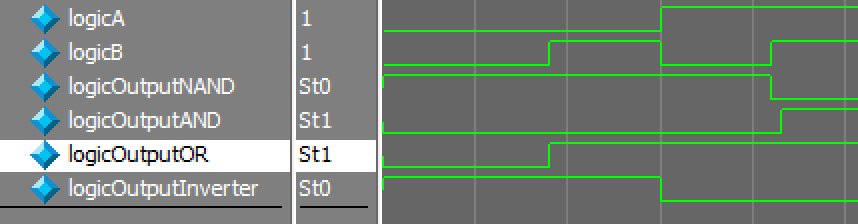
\includegraphics[width=.48\textwidth]{Images/LogicOutput.png}
      \caption{Example output of testbench}
    \end{figure}

    Take a moment to look at the simulation transcript, it provides the states of the logic elements being tested.
    I prefer having the simulator give a test listing instead of reading the waveforms. This is from the \$display()
    lines in the testbench. listing the outputs can be a very powerful debugging tool. I typically use the \$assert()
    statement, which will be explored below, which can execute two different blocks of code based on a logical test and alert you when an unexpected result is produced.
    \begin{lstlisting}
A:0 B:0 - Inverter:1 AND:0 OR:0 NAND:1
A:0 B:1 - Inverter:1 AND:0 OR:1 NAND:1
A:1 B:0 - Inverter:0 AND:0 OR:1 NAND:1
A:1 B:1 - Inverter:0 AND:1 OR:1 NAND:0
    \end{lstlisting}

  %| =================================================================================================
  %| Procedure: Verilog Testbench
  %| =================================================================================================
  \subsection{Verilog Testbench II}
    Verification is more than half the battle when working with Verilog. Mentor Graphics HDL simulator Modelsim is installed with Quartus. Modelsim is used extensively in logic design with Verilog. Fortunately Verilog offers a number of tools to make checking your code easier. The first of which is the assertion; it will run two different blocks of code depending on if a logical condition is met, It works much like an if statement that might be more familiar.
    \begin{lstlisting}[caption={Template for System Verilog assertion}]
//| This assertion will list an error if not met
assert (Logical statement)
  <code-for-true-case>
else
  <code-for-false-case>
    \end{lstlisting}

    The same code is used to test the adder from this lab's example code. The true case is used to display the valid output of the module. The false case throws a simulation error and shows the user the case. 
    \begin{lstlisting}[caption={Assertion Example from test bench}]
//| This assertion will list an error if not met
assert (Sum == SpecifiedConstant + Number)
  $display("Case %d: Pass", Number);
else
  $error("Case %d: FAIL:%d + %d /= %d", Number, Number, SpecifiedConstant, Sum);
    \end{lstlisting} 
    The logical statement in this code block checks to see if the output of the module is equal to the sum of specified constant and Number.Many designers write the test bench from specification in advance of the Verilog module. Testing should be an integral part of Verilog development from the beginning.

    All of the code from this first section is provided in source.zip. There is quite a learning curve to this part, be sure to watch the screen cast which describes the included modules. You will be assigned a constant by the lab instructor that the input number will be added to. This number should be entered as a parameter in the adder module's instantiation as is done in the test bench.

  %| =================================================================================================
  %| Procedure: 4-bit and constant adder 
  %| =================================================================================================
  \subsection{4-bit and Constant Adder Synthesis}
    The second section's adder will be synthesized and loaded onto the FPGA for this section. Use your dip switches and the LED circuits from the previous labs to test the adder for expected operation. This section is included with the example code, all you need to do is change the constant and test its operation.  

  %| =================================================================================================
  %| Procedure: 4-bit and 4-bit adder
  %| =================================================================================================
  \subsection{4-bit Full Adder Synthesis}
    This section requires the previous sections code to be modified to add two 4-bit inputs. This will require the removal of the previous modules' parametrization and the addition of an additional input port. 

  %| =================================================================================================
  %| Procedure: Comparator Design
  %| =================================================================================================
  \subsection{Design of Comparator}
    This section requires the previous sections code to be modified to add two 4-bit inputs. This will require the removal of the previous modules' parametrization and the addition of an additional input port. 

  %| =================================================================================================
  %| Procedure: Comparator Design
  %| =================================================================================================
  \section{Lab report}
    \IEEEPARstart{D}{ocumentation} is the most important part of an engineer's job. The sharper your writing skills the more employable you will be. Keep that in mind as you have to churn out documentation throughout college. This lab manual is written in almost textbook This particular lab report will require:
    \subsection{figures to include}
    \begin{itemize}
      \item Code listing of Full Adder
      \item Code listing for comparator
      \item It's important to remember Verilog is a Hardware Descriptive Language. The synthesis actually implements the Verilog in code. Quartus contains what are called ``Netlist Viewers'' that show the actual implementation. take a look at how Quartus synthesized your design as is shown in screencastX. Include screen captures of the combinatorial blocks listed in your design.
    \end{itemize}

    \subsection{Questions to Answer}
      \begin{enumerate}
        \item Do you think you would prefer the schematic design entry method of Lab two or the text based representation of this lab? In what situations do you think Schematic entry would be better, in which situations would Text base be advantageous.
      \end{enumerate}

  %| =================================================================================================
  %| Bibliography
  %| =================================================================================================
  \bibliographystyle{IEEEtran}
  \bibliography{IEEEfull}
\end{document}